\documentclass{article}

\title{Create your first Chrome extension}
\author{Bastien Boymond}
\date{}

\usepackage[utf8]{inputenc}
\usepackage[T1]{fontenc}
\usepackage{xcolor}
\usepackage{listings}
\usepackage{hyperref}
\usepackage{graphicx}

\graphicspath{ {../images/} }

\begin{document}
    \maketitle
    \begin{center}
        
\includegraphics[scale=0.1]{../images/chromeExtension.png}
    \end{center}
    \newpage
    \begin{description}
        \item[1 :]{Qu'est-ce qu'une extension Chrome ?} \\\\ Une \textbf{\href{https://chrome.google.com/webstore/category/extensions?hl=fr&authuser=0}{Extension Chrome}} est un addon qui permet d'ajouter des fonctionnalités à Chrome.
        \begin{center} 
            \rule{0.75\linewidth}{1pt}
        \end{center}
        \item[2 :]{Les dépendances}
\begin{lstlisting}[language=sh]
    sudo apt-get update
    sudo apt-get upgrade
    sudo apt-get install nodejs npm
\end{lstlisting}
        \begin{center} 
            \rule{0.75\linewidth}{1pt}
        \end{center}
        \item[3 :]{Créer un projet Chrome Extension}
\begin{lstlisting}[language=sh]
    mkdir chromeExtension
    cd chromeExtension
    npm init
\end{lstlisting}
        Une fois ça fais vous allez devoir Créer un fichier manifest.json et un fichier index.js.
        \\ Votre Manifest.json doit ressembler à ça :
        \begin{center}
            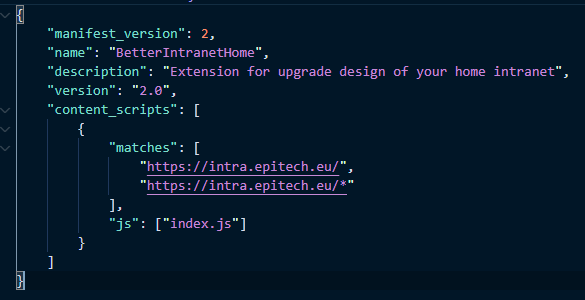
\includegraphics[scale=0.9]{../images/HowToManifest.PNG}
        \end{center}
        Actuellement vous avez fais une extension Chrome qui ne fait rien.
        Cette extension a seulement le droit de toucher au site de \textbf{\href{https://intra.epitech.eu/}{l'intranet}} C'est donc sur ce site que nous allons faire notre 1ere extension.
        \begin{center}
            \rule{0.75\linewidth}{1pt}
        \end{center}
        \item[4 :]{Tester votre extension Chrome} \\ Vous allez devoir tester votre extension Chrome. Pour cela il vous faut aller sur le site chrome://extensions/
        \\ Passez en mode Développer puis cliquez sur Charger l'extension non empaquetée.
        \begin{center}
            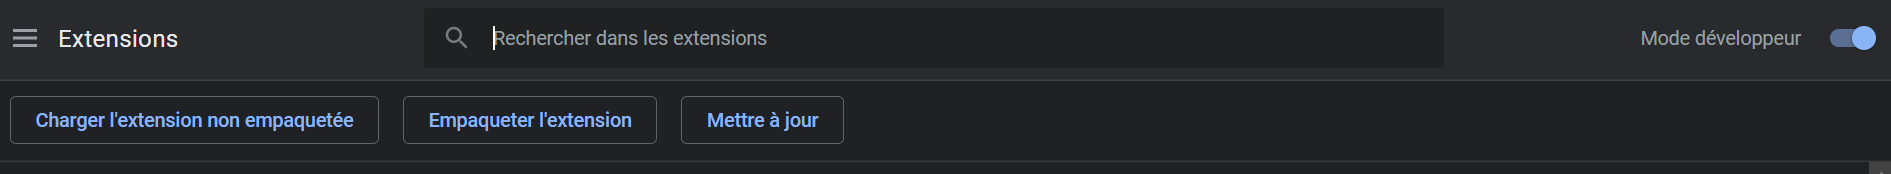
\includegraphics[scale=0.3]{HowToTestChorme.PNG}
        \end{center}
        Vous avez maintenant une extension qui fait rien.
        \begin{center}
            \rule{0.75\linewidth}{1pt}
        \end{center}
        \item[5 :]{Commencer à coder votre extension Chrome} \\ Maintenant que vous avez testé votre extension, vous allez pouvoir commencer à coder votre extension.
        \\ Notre objectif est de créer une extension qui affiche des informations sur la page home de l'intranet.
        \\ Pour cela nous allons chercher dans l'html de la page home de l'intranet l'endroit ci dessous :
        \begin{center}
            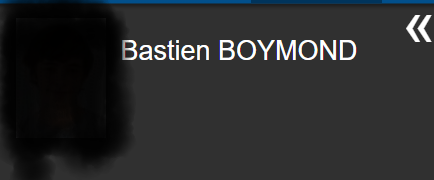
\includegraphics[scale=0.5]{FindInHtml.PNG}
        \end{center}
        Une fois trouvé nous allons créer une fonction qui va récupérer l'endroit en html correspondant à l'endroit que nous cherchons.
        \begin{center}
            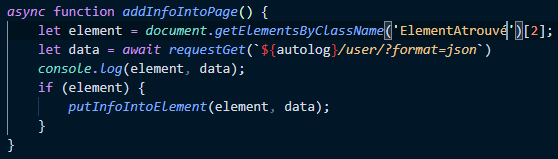
\includegraphics[scale=0.8]{indexjspremierePartie.PNG}
        \end{center}
        La variable element represente l'endroit que nous cherchons.
        \begin{center}
            \rule{0.75\linewidth}{1pt}
        \end{center}
        \item[6 :]{Récupérer la donnée que l'on veux rajouter à notre site} \\ Maintenant que nous avons récupéré l'endroit que nous cherchions nous allons récupérer la donnée dont nous avous besoin pour la rajouter à notre site.
        \\ Pour cela nous allons faire une requete avec l'API de l'intranet.
        \begin{center}
            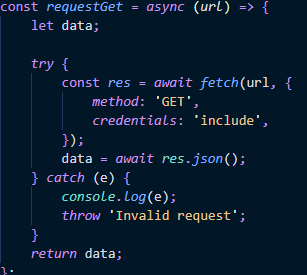
\includegraphics[scale=0.9]{requestGetSansLib.PNG}
        \end{center}
        L'url correspond à votre autologin que vous pouvez trouver à cette url : https://intra.epitech.eu/admin/autolog
        \\ Le lien ressemblera donc à une chose de ce genre : \\ \textbf{https://intra.epitech.eu/auth-f68d1af2174139ebceyvfde5646b4d/user/format=json} (L'autologin ici n'existe pas)
        \begin{center}
            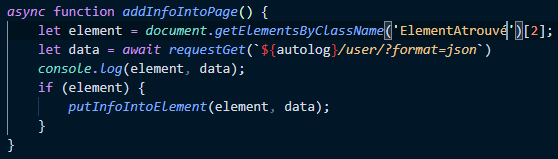
\includegraphics[scale=0.8]{indexjspremierePartie.PNG}
        \end{center}
        Maintenant que nous avons récupéré la donnée il est temps de la rajouter à notre site.
        \begin{center}
            \rule{0.75\linewidth}{1pt}
        \end{center}
        \item[7 :]{Rajouter la donnée à notre site} \\ Maintenant que nous avons toute les informations dont nous avons besoin nous allons rajouter la donnée à notre site.
        \\ Nous allons donc toucher à la fonction putInfoIntoElement créée plus tot.
        \\ Les taches à faire :
        \begin{itemize}
            \item Supprimer l'element <br>
            \item Trouver dans data ton Gpa, tes Crédits et ta promotion
            \item Ajouter la donnée dans l'element
        \end{itemize}
        Une fois fait le resultat doit ressembler à ça :
        \begin{center}
            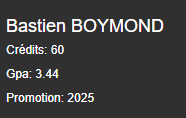
\includegraphics[scale=0.8]{final.PNG}
        \end{center}
        \item[8 :]{Pour aller plus loin} \\ Maintenant que nous avons rajouté la donnée à notre site nous allons pouvoir faire plus de choses.
        \\ Je vais vous proposer plusieurs choses à faire pour aller plus loin :
        \begin{itemize}
            \item Créer une popup qui affiche des informations d'epitech
            \item Mettre une image à votre extension
            \item Ajouter un bouton à votre extension qui vous inscrit à des projets
            \item Rendre le site web plus attractif
        \end{itemize}
    \end{description}
\end{document}